\documentclass[11pt, oneside]{article} 	% use "amsart" instead of "article" for AMSLaTeX format
\usepackage{geometry} 		% See geometry.pdf to learn the layout options. There are lots.
\geometry{letterpaper}  		% ... or a4paper or a5paper or ... 
\usepackage[parfill]{parskip} 		% Activate to begin paragraphs with an empty line rather than an indent
\usepackage{graphicx}				% Use pdf, png, jpg, or eps§ with pdflatex; use eps in DVI mode
								% TeX will automatically convert eps --> pdf in pdflatex		
\usepackage{amssymb}
\usepackage{amsmath}
\usepackage{authblk}
\usepackage[
backend=biber,
style=alphabetic,
]{biblatex}
\usepackage{graphicx}
\graphicspath{ {./images/} }
\usepackage{verbatim}
\usepackage{tikz} 
\usepackage{subfig}

\usepackage{syntonly}
% \syntaxonly <-- use this for checking syntax only
% \mbox {text} - keep together
% \fbox {text} - keep together and draw around

%\pagestyle{plain|headings|empty} % header and footer p.27
%SetFonts
%\include{filename}, \includeonly{filename1, filename2} , \input[fiename}

%SetFonts% 

\title{Solving N-dle using Information Entropy}
\author{Dave Fetterman}
\affil{Obviously Unemployed}
\date{6/19/22, Updated: 11/1/22}
\begin{document}
\maketitle

\begin{abstract}

This informal paper attempts to justify the use of information entropy as a solver heuristic for the expected value of guess count in a Wordle solution, to extend its use to its multiplexed cousins (Quordle, Octordle, and an abstracted n-dle), to practice my use of \LaTeX and Clojure, and to bore my friends.

\end{abstract}

\section{Introduction}

\emph{Note: This paper is a shameless tribute to and theft of Alex Healy's \textbf{On Optimal Strategies for Wordle}}\cite{1}. \emph{All credit to him and the nerd salon meeting in his Facebook comments for clarifying the debate about the best strategy for the game}.
 
\begin{figure}
\centering
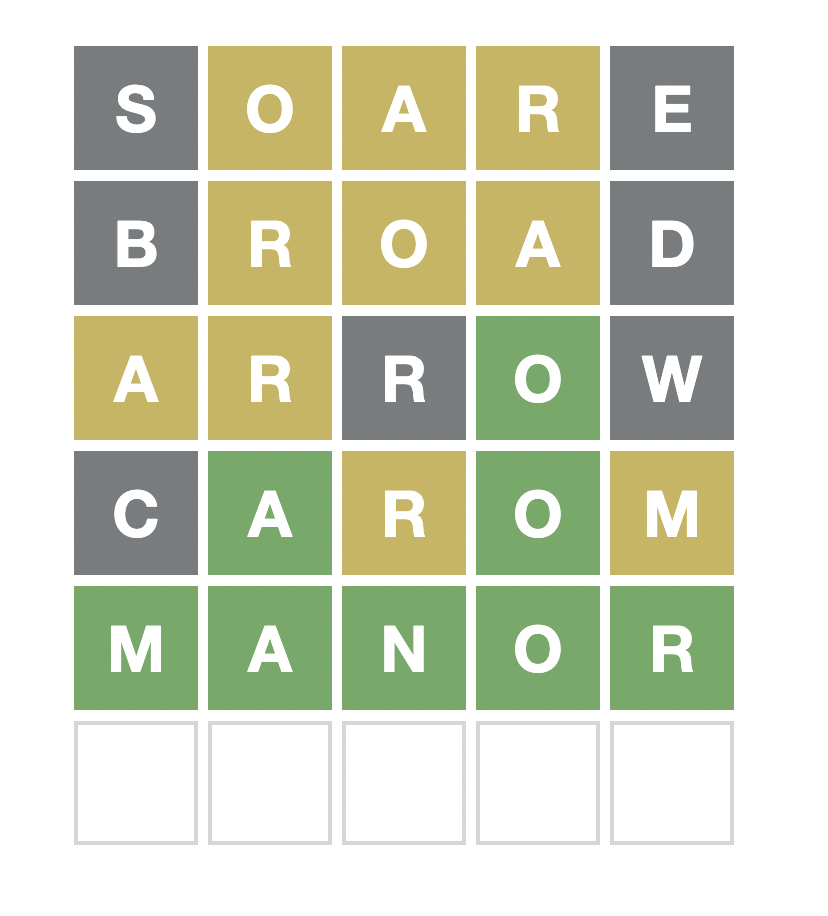
\includegraphics[scale=.3]{wordle}
\caption{An example finished Wordle board}
\end{figure}


For the likely reader, Wordle needs no introduction. The word game reskins the classic Mastermind with a restricted answer set (a highly reduced five-letter English word list) and restricted guess set (a larger five-letter English word list). The sharing and scarcity aspects of the game led to its viral spread, the creation of various knockoffs, and the app's purchase by the New York Times. If Pee-Wee's Word of the Day existed in 2022, this puzzle's solution would be it.

\subsection{Wordle Rules}
With six guesses to determine the hidden daily answer, each turn yields information from the oracle in the form of Green (G), Yellow (Y), and Black (B) squares. In response to a guess, five colored squares appear according to the rules in Fig. 2.


\begin{figure}
\centering
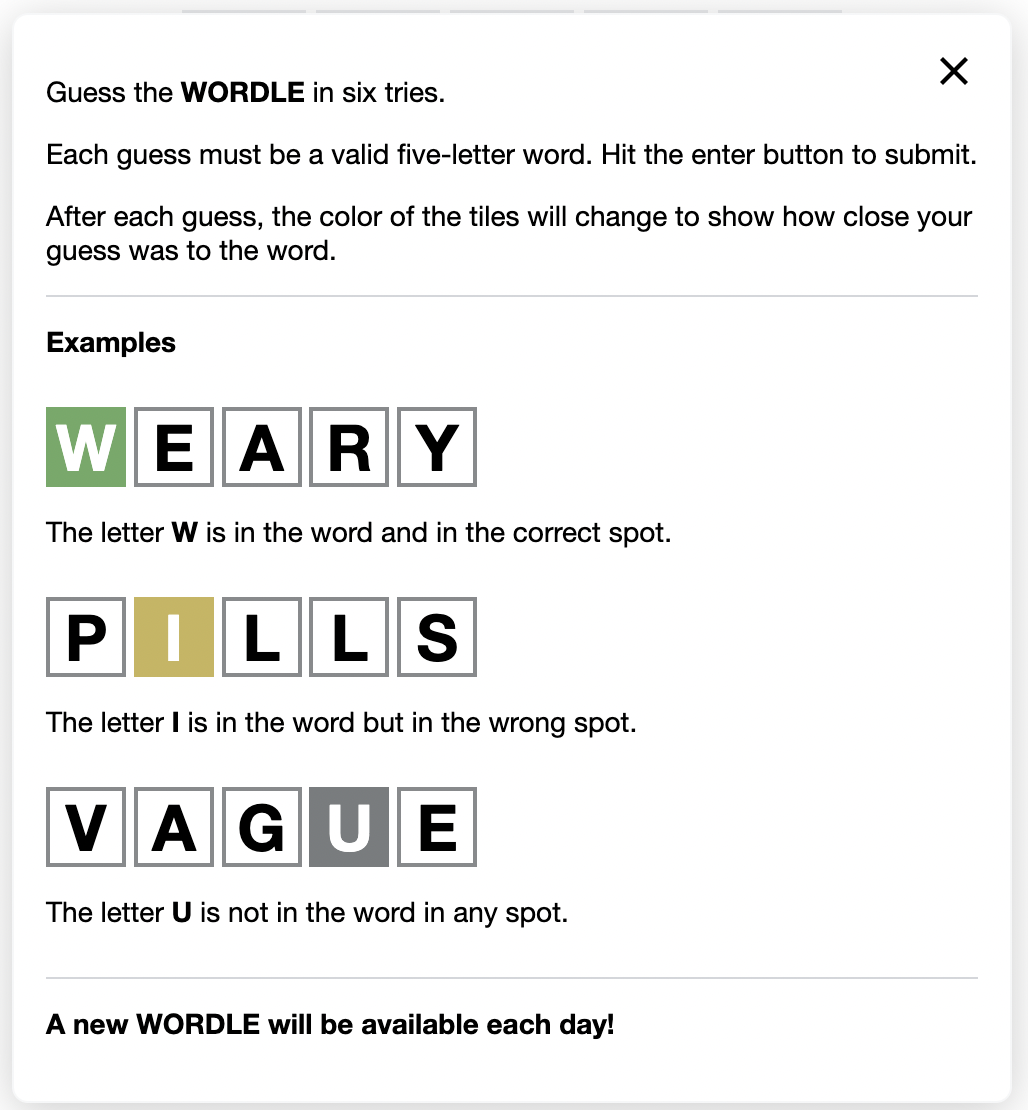
\includegraphics[scale=.5]{rules}
\caption{Official Wordle rules}
\end{figure}



If the solution has five unique letters, the above rules are straightforward to interpret. If the solution has repeated letters, note that, for any letter:

\begin{itemize}
\item The number of green and yellow squares returned for some letter, say A, don't exceed the number of instances of the letter A in the solution. (rule 1)
\item All yellow squares for some letter, say B, appear before all black squares for B. (rule 2) 
\end{itemize}
 
 As an example, if the answer is PASSE, and the guess is ASSES, the unique response will be YYGYB, not YYGYY (violates rule 1) or YBGYY (violates rule 2).


Starting with a fixed dictionary \footnote{Assumed here to be the 2309 words in \url{https://github.com/fettermania/wordle-solver/blob/main/wordle-answers.txt}}, the player has six guesses from an allowed guess list \footnote{The 12947 words in \url{https://github.com/fettermania/wordle-solver/blob/main/wordle-allowed-guesses.txt}} to enter the hidden answer word (that is, receive all greens as a response). Again, this is very similar to Mastermind \footnote{Note that "hard mode" Wordle, which has additional restrictions, is not treated here.}.

\subsection{Wordle Objective}

In Wordle, user gets a win if they can guess the hidden answer in six or fewer guesses, but given the social sharing in the game, bragging rights go to the solver who finishes in the fewest guesses. The task of optimizing guesses suggests different metrics (some unique to n-dle, $n > 1$), though these two seem ripest:

\begin{itemize}
\item The likelihood of finishing within six guesses.
\item The expected number of guesses required to finish.
\end{itemize}

At any stage of solving the puzzle, our state comprises the remaining guess count (starting from six and decrementing), the allowed guess list (an unchanging word list), and the solution dictionary (starting at the list of 2309 and successively filtered to only viable words given previous turns). It's then natural to ask:

\begin{itemize}
\item What's the best next guess at this point?
\item What's the best opening guess? This is a specific instance of the previous question with the entire word list and six guesses remaining.
\end{itemize}

This investigation employed an original solver and small test harness written to solve exactly these questions, aiming to minimize the expected guess count. \footnote{\url{https://github.com/fettermania/wordle-solver}}

\section{Information Entropy}

Among others, Alex Healy made the case \cite{1} for minimizing guess count using Claude Shannon's measure of Information Entropy \cite{2} as an evaluation heuristic for possible guesses at each stage. Entropy, though a powerful concept, seems fraught with different connotations connected in sophisticated ways. Among other definitions, entropy can mean:

\begin{enumerate}
\item Statistical randomness or disorder, especially in a physical system.
\item The amount of ``information content'' or ``surprising-ness'' of an event.
\item The minimum number of average bits required to specify a (string) message over a fixed probability distribution.
\item A specific function $H(E) = -\sum_{E_i \in E} \log_2(p_i)p_i$, over an event space $E$, where event $E_i$ has associated probability $p_i$, and further, which has these properties:
 \begin{itemize}
 \item $H$ is continuous over $p_1, ...,p_n$.
 \item If every $p_i = 1/n$, then $H$ increases monotonically with $n$.
 \item A composition law basically stating that renaming events through nested event spaces doesn't change the overall entropy of the set.
 \end{itemize}
\end{enumerate}

While the common definition (1) has an interesting connection to definition (3), and many papers use (2) as a shorthand, we will focus on definition (3) as motivation, and sometimes simply as a pure heuristic (4) with properties useful in Wordle.

Information entropy has a wide set of applications in computer networking, data science, and in general, communicating symbols, a place many of us find ourselves terminally and from which, not coincidentally, Wordle provides our brief escape.

\subsection{Entropy as minimum bits of message content}

Suppose a set of events E associates each member $E_i$ with a probability $p_i$. Loosely, suppose you need to communicate which of a set of events had occurred to a listener, who has no other information. The information entropy is then the expected value of the number of bits required to communicate that event over the prior probability distribution of the events.

I like to visualize this in in terms of Huffman tree variable-length encodings \cite{4}. Consider a language of three symbols (events) $E = \{A, B, C\}$, with likelihoods of occurring listed below, and the ideal encoding that falls out:

\begin{itemize}
\item A: encoding \texttt{0}, $p_a = \frac{1}{2}$
\item B: encoding \texttt{10}, $p_b = \frac{1}{4}$.
\item C: encoding \texttt{11}, $p_c = \frac{1}{4}$.
\end{itemize}

The average number of bits required to express a symbol is then 
$\frac{1}{2} \cdot 1 + \frac{1}{4} \cdot 2 + \frac{1}{4} \cdot 2 =\frac{3}{2}$.

It's not hard to see the form of $H(E) = -\sum_{E_i \in E} \log(p_i)p_i = \sum_{E_i \in E} \log(\frac{1}{p_i}) p_i$ here. If, instead, events C and D had probability $\frac{1}{8}$, encoding them (``locating it in the event space'') would each require $\log_2(8) = 3$ bits. It's clear in this case that the average length of the encoded message exactly corresponds to the entropy measure of this event space.

In this contrived example, where all events are independent and have probability of the form $2^{-n}, n \in \mathbb{N}$, the Huffman encoding is known to be optimal, and the average length of an encoding over this probability distribution is exactly Shannon's entropy measure \cite{4}.
 
\subsection{A Uniform distribution}

In first part of the last example, event A was twice as likely as B as well as C. An important case to consider is a \emph{uniform distribution}: when all $p_i$ are identical. If we were looking at communicating (encoding) one of the 2309 words in the Wordle dictionary as the answer, with all assumed to have equal probability, our entropy is then 

$H(E) = -\sum_{i=1}^{2309} \log_2(p_i)p_i = -\sum_{i=1}^{2309} \log_2(\frac{1}{2309}) \frac{1}{2309} = \log_2(2309) = 11.173$. 

This should not surprise. If you needed to communicate a message using 128 symbols with a uniform random distribution, you would need $\log_2(128) = 7$ bits for each. The ASCII encoding is one such example. But here, with about 4 more bits, you can encode not just a character but all words in the Wordle answer list!

If our dictionary of viable answers, filtered through learnings from previous guesses, is of size $m$, then our entropy measure of our answer set (filtered dictionary) at that point will be $\log_2(m)$, since each word is assumed equally likely. Notably, a single viable word remaining (a finished game) has entropy of $\log_2(1) = 0$. The solver's goal is to narrow its (filtered) dictionary to a single word, or, equivalently, to an event set with entropy zero.
 
\subsection{Applying entropy to Wordle}

Let us put probability aside for a moment and just think about playing Wordle to minimize our guess count.

As Alex Healy discusses \cite{1}, each guess in Wordle yields a colored tile response in $E = \{B, Y, G\}^5$, and partitions the possible answer words among those 243 sets (``events'')

\begin{center}
$E_{BBBBB}, E_{BBBBY}, E_{BBBBG}, ... , E_{GGGGG} \in E$. 
\end{center}

Again, if the guess is ASSES, the answer PASSE would be in $E_{YYGYB}$, and the answer ASSES would be in $E_{GGGGG}$.

If the dictionary were sufficiently reduced, (to say, 3 words), an ideal situation would see each such response set containing zero or one words. This means the next guess will either be a winner or eliminate two possibilities, producing a winner on the subsequent guess. 

The other end of the usefulness spectrum would be a guess with something like:
$|E_{BBBBB}| = 3$. Then, making this guess moves us no closer to the answer. 

Say our event space (dictionary) is E = \{\emph{dairy, brink, bring}\}. A guess of \emph{dairy} would yield the response set:

\begin{itemize}
\item $\{G, G, G, G, G\} \rightarrow (dairy)$.
\item $\{B, B, G, B, B\} \rightarrow (brink, bring)$.
\end{itemize}

One third of the time, we finish the game, and two thirds, we must navigate through a set of 2, which takes an average of $\frac{3}{2}$ more guesses. 

If, instead, we guessed \emph{brink}, our response set would be:
\begin{itemize}
\item $\{G, G, G, G, G\} \rightarrow (brink)$.
\item $\{G, G, G, G, B\} \rightarrow (bring)$.
\item $\{B, B, G, B, B\} \rightarrow (dairy)$.
\end{itemize}

In this case, we either get our guess right or have a set of one to land on.

It's no surprise that, we prefer the second scenario; therefore, \emph{brink} (or \emph{bring}) is the appropriate guess here. It is here that we connect to the entropy measure.

\subsection{Defining Wordle response set entropy}

We're going to measure the effectiveness of any given guess across the current dictionary by looking at the distribution of possible dictionary states after executing the guess. Some of these states will bring us right to an answer, while some will leave us with a dictionary not much reduced from our current one. We are looking to optimize the average entropy of the remaining dictionary given our guess.

\begin{center}
$H(solution | guess) = \sum_{i \in \{B, Y, G\}^5} \log(1/ p_i) p_i$.
\end{center}

However, how should we define $p_i$ in this case? Consider that, at any point of the game, all remaining words are equally likely to be the solution. Then, the chance that the answer is in set $E_i$ is its proportion of the remaining dictionary $E$ ($|E| =\sum_{i \in \{B, Y, G\}^5} |E_i|$), or $p_i = \frac{|E_i|}{|E|}$. This renders our entropy measure as :

\begin{align}
H(E | g) = \sum_{i \in E} \log(\frac{1}{p_i}) \cdot p_i \\
= \sum_{i \in E} \log(\frac{|E|}{|E_i|}) \cdot \frac{|E_i|}{|E|} \\
= \sum_{i \in E} (\log(|E|) - \log(|E_i|)) \cdot \frac{|E_i|}{|E|} \\
= \sum_{i \in E} \log(|E|) \cdot \frac{|E_i|}{|E|} - \sum_{i \in E}\log(|E_i|) \cdot \frac{|E_i|}{|E|} \\
= \log(|E|) \sum_{i \in E} \cdot \frac{|E_i|}{|E|} - \sum_{i \in E}\log(|E_i|) \cdot \frac{|E_i|}{|E|} \\
= \log(|E|) - \sum_{i \in E}\log(|E_i|) \cdot \frac{|E_i|}{|E|}
\end{align}

This measure (6) was used in Alex Healy's paper \cite{1} in a different form (I'll name it (7)), written simply as:
\begin{center}
$H(solution | guess) = \sum_{i \in E}\log(|E_i|) \cdot \frac{|E_i|}{|E|}$ 
\end{center}

In this case, a (highly desired) response set in which every $E_i$ contained at most one word would necessarily be of $zero$ entropy, while (6) would yield maximal entropy $\log(|E|)$. What gives?

Entropy (6) characterizes the bits required to communicate an event among many outcomes, or the \emph{entropy the oracle gives up in yielding its response}. The Wordle metric (7) represents an expected value of \emph{how much entropy remains}. For any $E_i$, the entropy (number of bits required to communicate a member of this uniformly distributed set) is $\log(|E_i|)$, so the measure falls out readily. Then, we seek to maximize the information given up by the response (6) in order to get (7) as close to 0 as possible. These metrics differ by a constant factor, which doesn't interfere with combining entropies together (which we'll do later), but this clarification helps me conceptualize why, using one equation a maximally entropic (spread out) solution set is desired, while in another form, we push our total entropy to zero.

\section{Applying entropy to Wordle}

The greedy algorithm for solving Wordle with answer list E and viable guess list G using entropy is straightforward:
\begin{enumerate}
\item If E is of size 1, exit with answer.
\item For each $g \in G$: 
 \begin{enumerate}
 \item For each $a$ in E, compute which response set $E_i$ (for example, $E_{YYGYB}$) each answer $a$ would fall into given guess $g$.
 \item Compute $H^*(E | g)$, where $H^* = -100$ if $|E| = 1$, else $H^* = H$ from form (7) above \footnote{This -100 encourages selecting a viable answer on the next guess (filtered dictionary of size one, entropy zero) over a larger set of entropy zero which solves in two guesses.}
 \end{enumerate}
\item Choose the $g$ that minimizes $H^*(E | g)$. \footnote{Should guesses see ties for lowest entropy, the algorithm should either take a deterministic stance (e.g. first alphabetical) or a fair one (random selection), depending on the goals of the investigation.}
\end{enumerate}

\subsection{Initial entropies for first subpuzzle solved}

The starting entropies for a full dictionary of 2309 words are listed below. (Words in the answer list are in bold)

Since we start at an identical state for each board (2309 words remaining), the entropies for legal first subpuzzle solvedes below occur for all games of Wordle, as well as n-dle versions we will see shortly. \textbf{Bold} guesses indicate those in the answers list.
\begin{center}
\begin{tabular}{ |c|c|c| }
 \hline
word & post-guess entropy \\
\hline
soare & 5.287849713481362 \\
roate & 5.288196144042106 \\
\textbf{raise} & 5.294749501280944 \\
reast & 5.305314436930554 \\
raile & 5.307898628732849 \\
\textbf{slate} & 5.317233213664601 \\
salet & 5.337029675681638 \\
\textbf{crate} & 5.337836475140834 \\
\textbf{irate} & 5.34025357683321 \\
\textbf{trace} & 5.342623349694359 \\
\hline
\end{tabular}
\end{center}

Because the algorithm is entirely deterministic, the solution of each of the 2309 Wordle puzzles (completely specified by the answer word) necessarily started with \emph{soare}.

\subsection{Results of Greedy Entropy algorithm for Wordle (1-dle)}

Since there are only 2309 possible games of Wordle, we can simulate each game using the greedy algorithm with entropy heuristic to see its performance.

\begin{center}
\begin{tabular}{ |c|c|c| }
 \hline
guesses & count & proportion \\
 \hline
2 & 22 & 0.0095 \\
3 & 888 & 0.3846 \\
4 & 1298 & 0.5621 \\
5 & 99 & 0.0429 \\
6 & 2 & 0.0009 \\
 \hline
\end{tabular}
\end{center}

\begin{figure}%
 \centering
 \subfloat[\centering guesses required]{{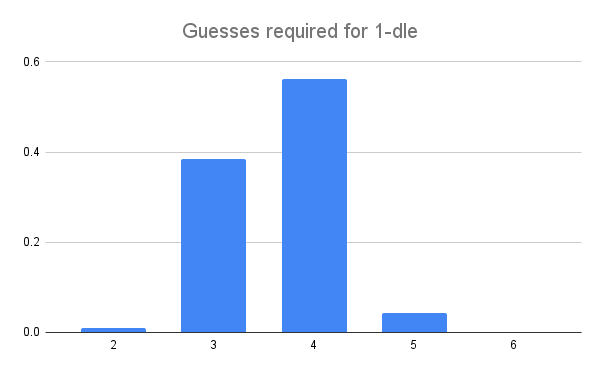
\includegraphics[scale=.33]{guess1} }}%
 \qquad
 \subfloat[\centering frequency of openers]{{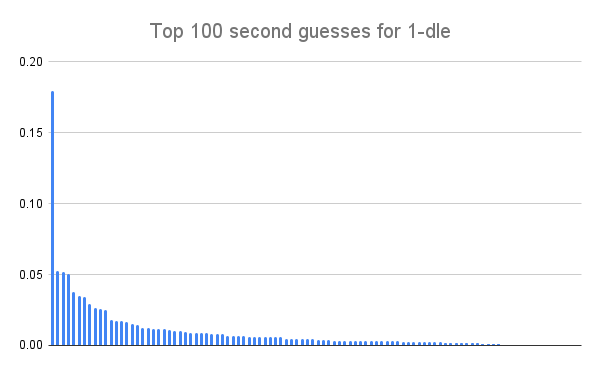
\includegraphics[scale=.33]{second1}}}%
 \caption{1-dle (Worlde) results on all 2309 answers}%
\end{figure}


\begin{itemize}
\item Expected Guess Count: 3.640970117
\item Opener 1: \emph{soare, clint} (0.1797314855)
\item Opener 2: \emph{soare, thilk} (0.05283672586)
\item Opener 3: \emph{soare, denet} (0.0515374621)
\item Opener 4: \emph{soare, tined} (0.05067128627)
\item Prevalence of top four openers \footnote{Four chosen somewhat arbitrarily, but where the curve bends strongly.} openers: (0.3347769597)
\end{itemize}

These results are very similar to Healy's results on a dictionary of 2315 \cite{1}, with some moderate differences \footnote{On correspondence, Healy has a better strategy for favoring dictionary guesses on ties}. Of note is that all words are solvable in six guesses (the maximum allowed for the game), the average word takes about 4 guesses to pin down, and the top four second guess (post-\emph{soare}) words only constitute about a third of the optimal plays. We will revisit these numbers later.

\subsection{Entropy advantages}

The faults with this algorithm are expected. 
\begin{itemize}
\item Although guesses are commutative (playing words in different orders yields the same filtered dictionary), since not every word is playable (unlike Mastermind), optimizing for only the next guess may miss a more globally optimal solution. More generally, it is not obvious to me that minimizing the entropy measure minimizes the expected value of guesses remaining in all cases. 
\item If we are optimizing to get under, say, six guesses, choosing a guess with ``maximal information'' that's not in the answer list may still be suboptimal compared to a shot at an answer.
\end{itemize}

\textbf{However, one major advantage of the entropy approach is the easy scale when expanding the game to multiple independent boards, as in Wordle derivatives Quordle (4 boards) and Octordle \footnote{I often refer to these as 4-dle and 8-dle, respectively, my own shorthand.} (8 boards)}. Via entropy, we can calculate a candidate guess's effectiveness on each board's answer dictionary, and then look for the minimum summed entropy across all boards. With N boards, this means we can do calculations on $|G|\cdot N$ possibilities (calculate board's entropy for each guess on every board) than $|G|^N$ (consider every possible N-tuple of answers).

\section{N-dle using entropy}

\begin{figure}[!htb]
\centering
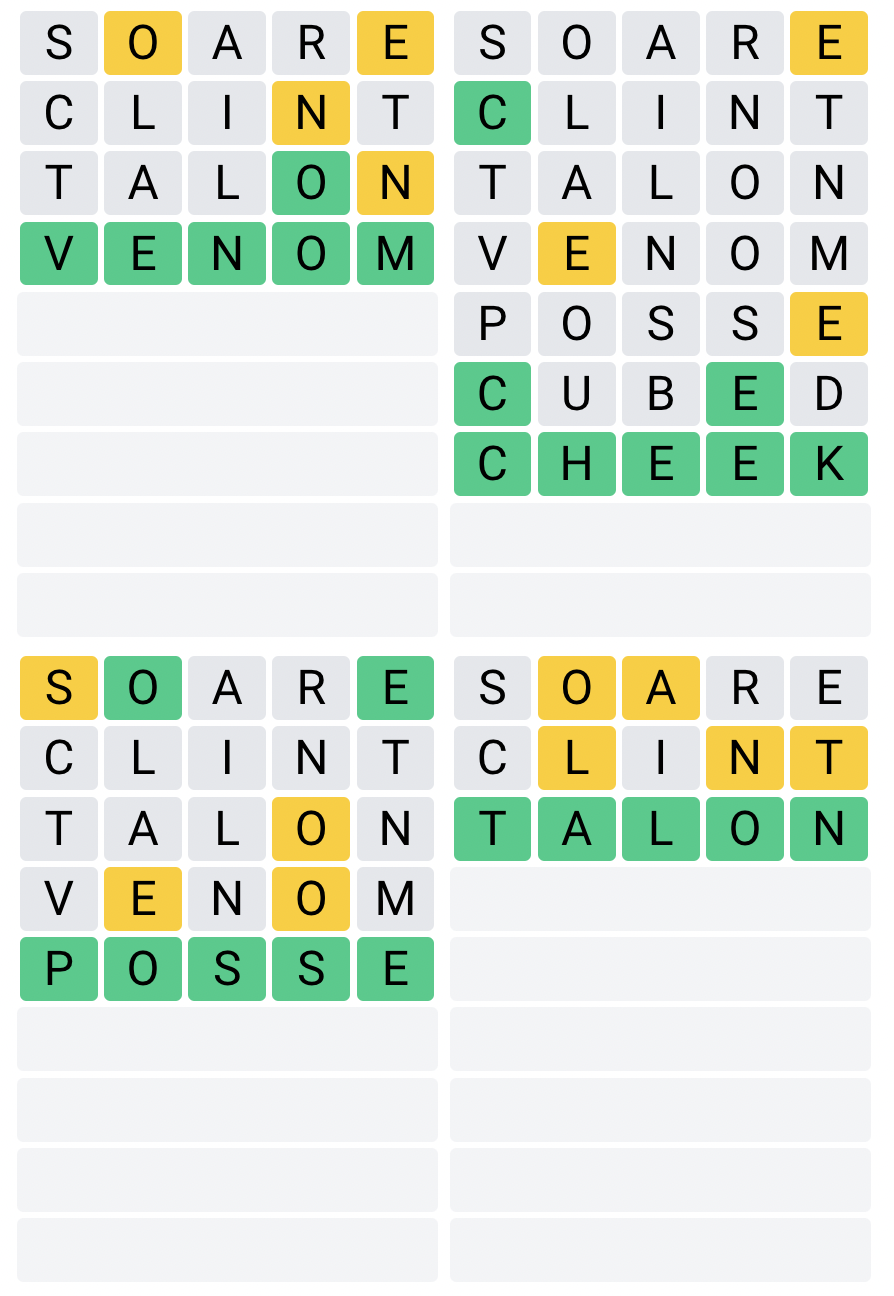
\includegraphics[scale=.3]{quordle}
\caption{Example Quordle board}
\end{figure}


While in 1-dle (Worlde) we've defined our events $E_i$ in a way such that, on one guess, they can never co-occur, using entropy as the scoring function starts to make even more sense when considering two independent boards. Here, take X to be the (uniform) distribution of possible remaining answers on one Wordle board with a secret answer $a_x$, and Y to be another with an independently chosen answer $a_y$. Note that the legal guess set G does not change across turns or boards.



If we consider a ``response'' function $R(g, a)$ which takes a guess and an answer and outputs a color-tuple response $r \in \{B, Y, G\}^5$, it should be clear that knowing $R(g, X)$ yields no information about $R(g, Y)$ (and vice versa). If a guess $g$ has some probability $p_i$ of ending up in set $X_i$, that's only because there are $p_i = \frac{|X_i|}{|X|}$ remaining answers $a$ in $X$ in which $R(g, a) \in X_i$, and similarly for $p_j$ in every set $Y_j$. The choice of $a_x$ and $a_y$ are independent, and therefore, these variables are as well.

Since $X$ and $Y$ are independent, the entropy of their joint distribution is the sum of the entropies of the individual distributions. This is a known result \cite{3} but also falls out of the composition requirement for entropy.


\textbf{We've argued that this pairwise independence is true for two boards, and it logically can be extended to three, four (quordle), eight (octordle), and so on.} This means we can look at a similar algorithm for ``N-dle'':

\begin{enumerate}
\item If there are no unsolved boards, exit.
\item For each board n of board set N:
 \begin{enumerate}
 \item For each $g \in G$: 
 \begin{enumerate}
 \item For each $a$ in $E_n$, compute which response mask set $E_{n_i}$ (for example, $E_{YYGYB}$) each answer $a$ would fall into given guess $g$.
 \item Compute $H^*(E_n | g)$, where $H^* = -100$ if $|E_n| = 1$, is 0 if $|E_n| = 0$, else $H^* = H$ from form (7) above. \footnote{This means that we're going to immediately solve any boards of dictionary size 1, always a correct guess for minimizing our expected value. To see that's true, commute that guess with a non-solving guess! And if you are solving 10+ puzzles at once, feel free to magic up this -100 number appropriately.}
 \end{enumerate}
 \item Choose the $g$ that minimizes $\sum_{n}H^*(E_n | g)$ 
\end{enumerate}
\end{enumerate}

Note that, because our measure $\sum_{n}H^*(E_n | g)$ is the sum of the entropy measures from Wordle (1-dle), the minimum entropy word starting from a full dictionary (\emph{soare}) also minimizes this summed entropy. So, every simulation in this whole paper therefore opens with guess \emph{soare}.

\section{Experimental Results for N-dle}
For 2-dle and beyond, computing the best path through $2309^n$ possibilities quickly becomes untenable. So, for this (as well as 4-dle and 8-dle), we settle for a simulation of 10000 random board sets. 
Note that these may not correspond exactly to a the distribution of Quordle or Octordle proper, as (a) this is a random sampling of a large space, and (b) simultaneous duplicate answers may occur in our simulation \footnote{Our technique of summing entropies requires independence between two or more distributions, so we have to include duplicates in the answer space.} but are likely not included in the public Quordle or Octordle apps.


\subsection{2-dle}

\begin{figure}[!htb]
 \centering
 \subfloat[\centering guesses required]{{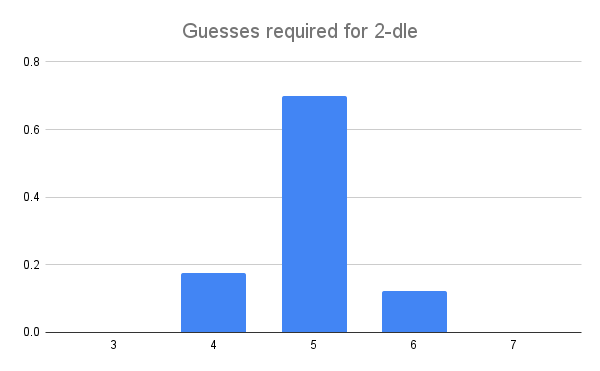
\includegraphics[scale=.33]{guess2} }}%
 \qquad
 \subfloat[\centering frequency of openers]{{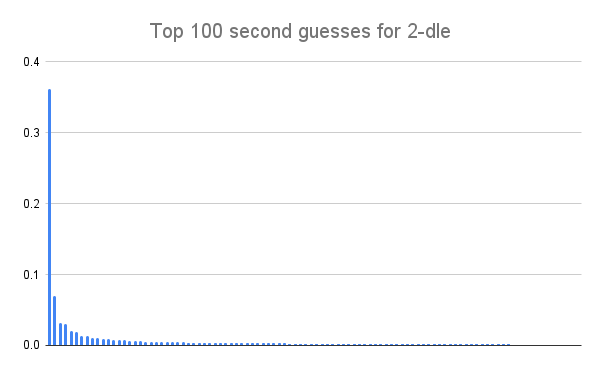
\includegraphics[scale=.33]{second2}}}%
 \caption{2-dle results on 10000 random answer sets}%
\end{figure}

\begin{center}
\begin{tabular}{ |c|c|c| }
 \hline
guesses & count & proportion \\
 \hline
3 & 11 & 0.0011 \\
4 & 1766 & 0.1766 \\
5 & 6981 & 0.6981 \\
6 & 1219 & 0.1219 \\
7 & 23 & 0.0023 \\
 \hline
\end{tabular}
\end{center}

\begin{itemize}
\item Expected Guess Count: 4.9477
\item Opener 1: \emph{soare, clint} (.3613)
\item Opener 2: \emph{soare, clipt} (.0699)
\item Opener 3: \emph{soare, linty} (.0317)
\item Opener 4: \emph{soare, mulct} (0.0304)
\item Prevalence of top four openers: (0.4933)
\end{itemize}

A few observations from this data:
\begin{itemize}
\item Again, if N is the number boards (here $N=2$), all answers are solvable within N+5, with the mean around N+3.
\item The distribution of guesses has started to tighten around this mean. 
\item The opener of \emph{soare, clint} accounts for over a third of our solver's paths in 2-dle, more than sum of the top four of 1-dle. 
\end{itemize}


\subsection{Quordle (4-dle)}

Unlike 2-dle \footnote{\url{twodle.net} appears to be a game but without the same setup as Quordle or Octordle. The user ventures not one but two guesses for two separate boards}, Quordle is a playable game available on the internet. The question of how to solve it within 9 moves (cover lots of letters in the first few guesses? solve the most favorable sub-board aggressively?) does not have an obvious answer. However, when looking at how our solver approaches the problem, it unsurprisingly appears to favor the strategy of gathering information across all boards, and going for the throat only when the answer is clear.

\begin{figure}[!htb]
 \centering
 \subfloat[\centering guesses required]{{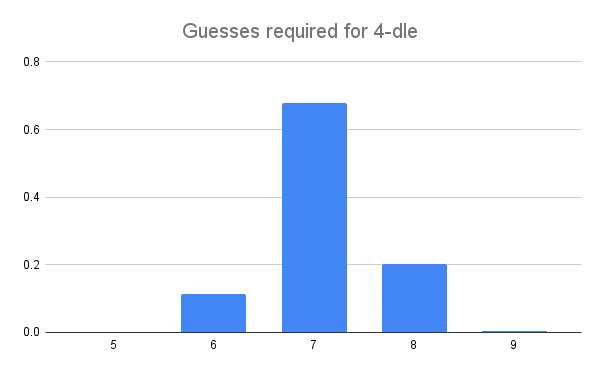
\includegraphics[scale=.33]{guess4} }}%
 \qquad
 \subfloat[\centering frequency of openers]{{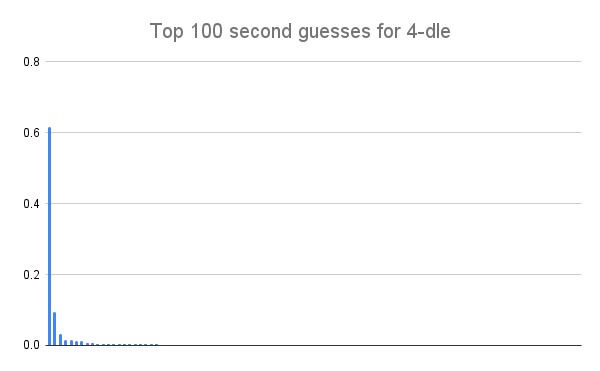
\includegraphics[scale=.33]{second4}}}%
 \caption{4-dle (Quordle) results on 10000 random answer sets}%
\end{figure}

\begin{center}
\begin{tabular}{ |c|c|c| }
 \hline
guesses & count & proportion \\
 \hline
5 & 6 & 0.0006 \\
6 & 1146 & 0.1146 \\
7 & 6776 & 0.6776 \\
8 & 2032 & 0.2032 \\
9 & 40 & 0.004 \\
 \hline
\end{tabular}
\end{center}


\begin{itemize}
\item Expected Guess Count: 7.0954
\item Opener 1: \emph{soare, clint} (0.6166)
\item Opener 2: \emph{soare, clipt} (0.0942)
\item Opener 3: \emph{soare, mulct} (0.032)
\item Opener 4: \emph{soare, linty} (0.0167)
\item Prevalence of top four openers: (0.7595)
\end{itemize}

Observations: 
\begin{itemize}
\item All answers are solvable within N+5, with the mean around N+3, a consistent pattern so far.
\item The distribution of guesses remains tight around the mean, though less so than our 2-dle simulation.
\item The opener of \emph{soare, clint} accounts for nearly \emph{two} thirds of our solver's paths in 4-dle, almost double that of 2-dle. The opener frequency graphs from here on out are dramatically long-tailed.
\item We see a lot of familiar faces among the top four openers (clint, clipt, mulct, linty), a rearrangement of the 2-dle headliners.
\end{itemize}


\subsection{Octordle (8-dle)}

Our final simulation occurred on 8 simultaneous boards. Because the algorithm has linear runtime over the board count N, we could continue, though 10000 simulations proved time-consuming, and the patterns have established themselves clearly at this point. 

\begin{figure}[!htb]
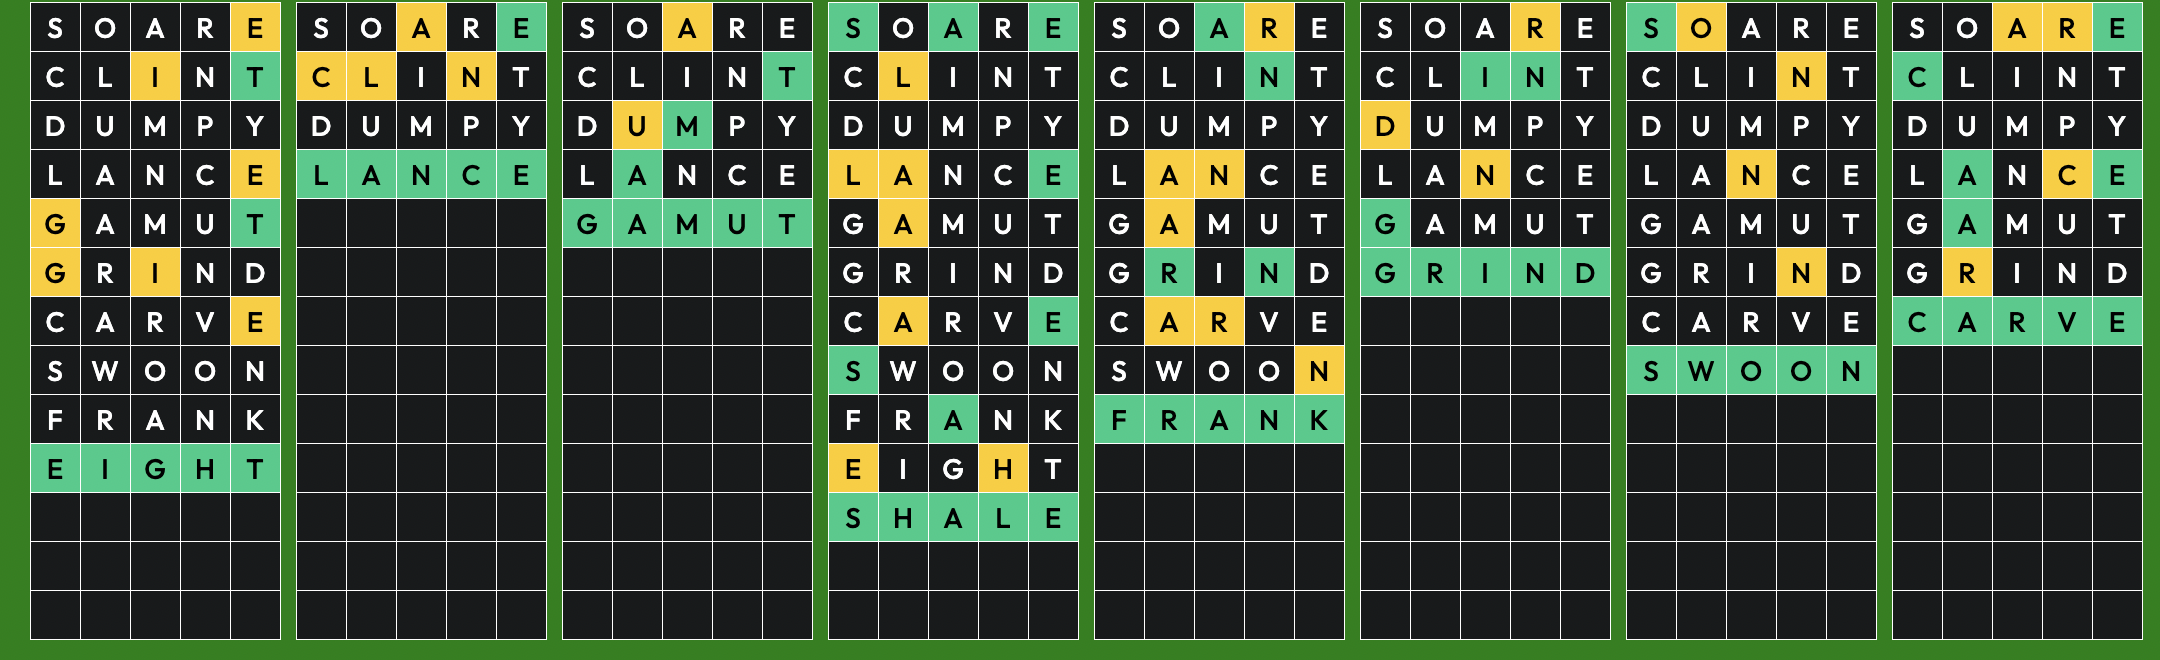
\includegraphics[scale=.33]{octordle}
\caption{Example Octordle board}%
\end{figure}

\begin{figure}[!htb]
 \centering
 \subfloat[\centering guesses required]{{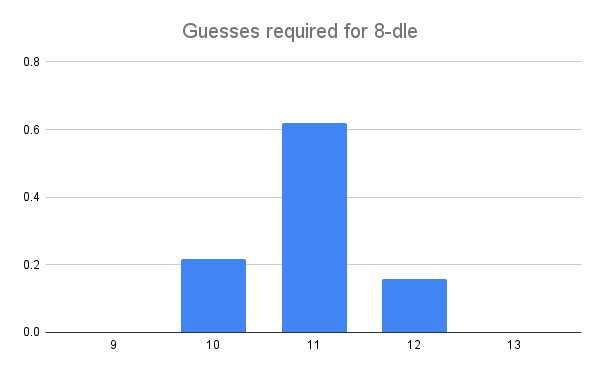
\includegraphics[scale=.33]{guess8} }}%
 \qquad
 \subfloat[\centering frequency of openers]{{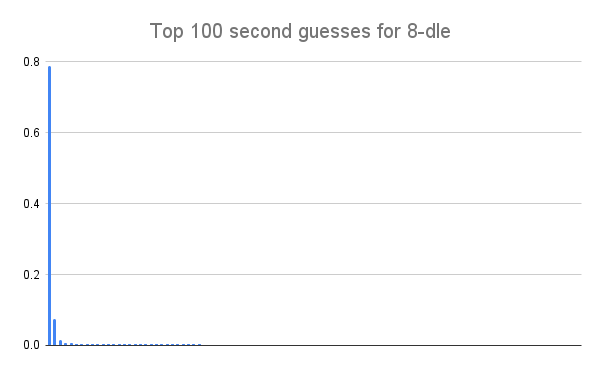
\includegraphics[scale=.33]{second8}}}%
 \caption{8-dle (Octordle) results simulated on 10000 answer sets}%
\end{figure}

\begin{center}
\begin{tabular}{ |c|c|c| }
 \hline
guesses & count & proportion \\
 \hline
9 & 19 & 0.0019 \\
10 & 2182 & 0.2182 \\
11 & 6202 & 0.6202 \\
12 & 1571 & 0.1571 \\
13 & 26 & 0.0026 \\
 \hline
\end{tabular}
\end{center}

\begin{itemize}
\item Expected Guess Count: 10.932
\item Opener 1: \emph{soare, clint} (0.7888)
\item Opener 2: \emph{soare, clipt} (0.0745)
\item Opener 3: \emph{soare, mulct} (0.0162)
\item Opener 4: \emph{soare, glint} (0.0072)
\item Prevalence of top four openers: (0.8867)
\end{itemize}

Observations: 
\begin{itemize}
\item All answers are solvable within N+5, with the mean around N+3. 
\item The opener of \emph{soare, clint} accounts for three quarters of our solver's paths in 8-dle.
\item The relevance of optimal starters after \emph{soare, clint} continues to drop. 
\end{itemize}

\section{Trends and Traps}

A few trends seem to emerge from these results across 1-, 2-, 4-, and 8-dle. 

As N increases:
\begin{itemize}
\item The solver seems to gravitate to a universal second-word opener in \emph{clint}, provided we don't stumble upon one of the 22 immediate solves (see 1-dle results section). This resonates with the ``law of large numbers" intuition \footnote{possibly wrong} that, as N increases, the "best fit" guess would only fit better.
\item The mean solution seems stuck at about N+3 so far. Given that two non-answers (\emph{soare}, \emph{clint}) constitute most of the openers, this means we're looking at either one more clarifying non-answer or one wrong answer guess on average. This could be clarified with some more logging in the solver.
\item Almost all puzzles are solved in N+4 guesses, and a few in N+5. Considering that 6, 9, and 13 are the guess limits in Wordle, Quordle, and Octordle, respectively, it seems the game designers have noticed this also.
\end{itemize}
 
However, consider the thought experiment of a 2309-word board (if chosen randomly, duplicates become a near-certainty).
\begin{itemize}
\item The first subpuzzle solved of the non-answer \emph{soare} would almost certainly be inferior to actual possible answer \emph{raise}. \emph{raise} has a 63.2 percent chance \footnote{$\approx 1- e^{-1}$} of being in the puzzle, and its shortfall of .01 bits of entropy \footnote{Although, on second look the shortfall is more like 2309 * .01 = 23 bits. Just what is eliminating a bit of entropy worth?} likely is worth less than solving an average of one sub-puzzle.
\item The maximum solution length (N) falls out of the definition, though 2309 unique sub-boards occur together with vanishing probability.
\item One suspects that the average solution length would trend from N+3 (where it seems stuck so far) to far below N, the chance of a zero-entropy sub-puzzle emerging at every turn. More directly, the expected portion of the answer list represented in the boards becomes $\frac{1}{2309} \sum_1^{2309} (1 - (\frac{2309 - 1}{2309})^{2309}) \approx 1 - e^{-1} = .632$ \footnote {You again.}, in which case we're solving a 1459-dle!
\end{itemize}

These generalizations follow from the observations, which could also be wrong as I broke entropy ties arbitrarily, using the internal sorting of Clojure (or possibly JVM). Ties really should have been broken randomly (for estimating mean) or, say, alphabetically (for cataloguing ``best words''). However, this whole paper remains an exploration of just one algorithm among many anyway.

\section{An Alternative Algorithm: Vern's Gambit}

Finally, note that the algorithm detailed here not the only strategy, nor even the only strategy relying on \emph{entropy}! Another greedy algorithm solves Wordle with answer list E and viable guess list G using entropy, but looks to minimize the minimum entropy of the unsolved sub-puzzles.  The algorithm:
\begin{itemize}
\item If there are no unsolved boards, exit.
\item For each board n of N:
 \begin{itemize}
 \item For each $g \in G$: f
 \begin{itemize}
 \item For each $a$ in $E_n$, compute which response mask set $E_{n_i}$ (for example, $E_{YYGYB}$) each answer $a$ would fall into given guess $g$.
 \item Compute $H^*(E_n | g)$, where $H^* = -100$ if $|E_n| = 1$, $H^* = 0$ if $|E_n| = 0$, else $H^* = H$ 
 \end{itemize}
 \item Choose the $g$ associated with the lowest entropy $H^*(E_n | g)$ in any board. 
\end{itemize}
\end{itemize}

This algorithm, named \emph{Vern's Gambit} (or the \emph{min strategy}), greedily chases the most promising sub-puzzle (that with the minimum individual board entropy) instead of optimizing for the total entropy of the entire system as described in Section 3. The Section 3 algorithm is called the ``sum method'' from here on out.

It is indistinguishable from the main algorithm in a few cases:
\begin{itemize}
\item When $n = 1$ (Wordle), these are exactly the same algorithm.
\item When a board (say a single one) is solvable on the next move, the main algorithm will see a minimum total entropy\footnote{Again, $-100$ is meant to signify ``negative infinity'' and should be increased or coded more logically as needed.}  of $-100$ plus the much smaller entropies of unsolved boards. The min algorithm simply sees $-100$. Each will make the same selection.
\end{itemize}

However, the data for the min method bears out major differences:
\begin{itemize}
\item Exhibiting higher risk-taking (variance), the maximum number of guesses for a full puzzle greatly exceeds that of the ``sum method''.
\item The average guess count to solve a puzzle is higher. In 2-, 4-, and 8-dle, this is about a half-guess. 
\item When compared head-to-head (that is, on the same puzzle), the sum method appears more effective as N increases.
\item The concentration of common openings (first two words) dilutes considerably as the individual puzzles exert a strong influence on the next move with minimum entropy.
\item As a sanity check, the number of guesses required to find the first sub-puzzle solution (the algorithm's natural goal) appears slightly smaller with the min method. As the algorithm explicitly seeks this out, this result seems intuitive.
\end{itemize}



\subsection{2-dle under Vern's gambit}

\begin{center}
\begin{tabular}{ |c|c|c| }
 \hline
guesses & count & proportion \\
 \hline
3 & 11 & 0.0011 \\
4 & 1296 & 0.1296 \\
5 & 5279 & 0.5279 \\
6 & 3171 & 0.3171 \\
7 & 242 & 0.0242 \\
8 & 1 & 0.0001 \\
 \hline
\end{tabular}
\end{center}


\begin{figure}[!htb]
 \centering
 \subfloat[\centering guesses required]{{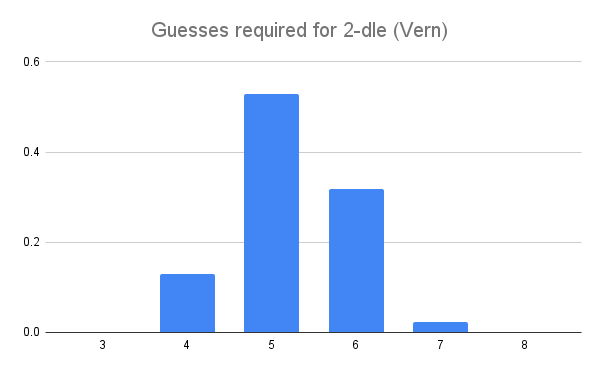
\includegraphics[scale=.33]{guess2_vern} }}%
 \qquad
 \subfloat[\centering frequency of openers]{{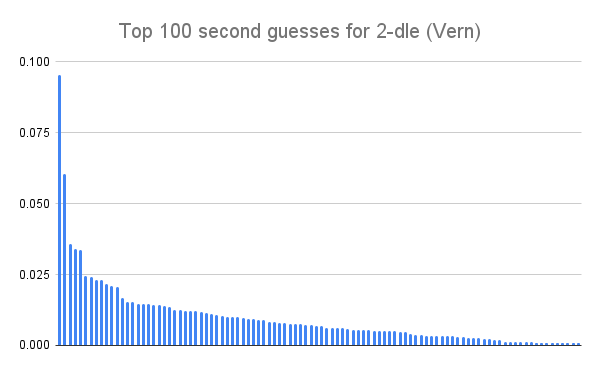
\includegraphics[scale=.33]{second2_vern}}}%
 \caption{2-dle results on 10000 random answer sets (Vern)}%
\end{figure}

\begin{figure}[!htb]
 \centering
 \subfloat[\centering last subpuzzle solved]{{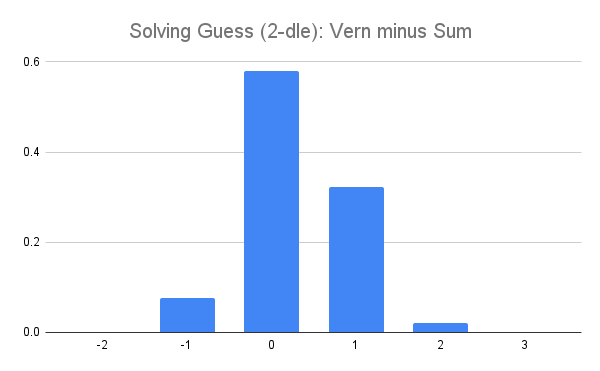
\includegraphics[scale=.33]{last_guess_comparison_2} }}%
 \qquad
 \subfloat[\centering first subpuzzle solved]{{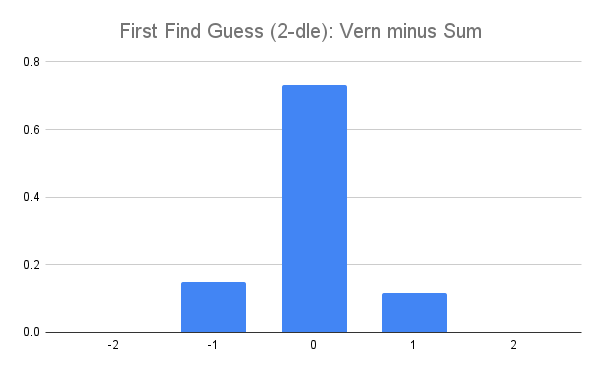
\includegraphics[scale=.33]{first_guess_comparison_2} }}%
 \caption{Comparison of Vern and Sum algorithms on 2-dle}%
\end{figure}


\begin{itemize}
\item Expected Guess Count: 5.234 (vs. sum strategy: 4.9477)
\item Opener 1: \emph{soare, clint} (.0955)
\item Opener 2: \emph{soare, thilk} (.0604)
\item Opener 3: \emph{soare, cloot} (.0358)
\item Opener 4: \emph{soare, denet} (0.0341)
\item Prevalence of top four openers: (0.2258). 
\end{itemize}

A few observations on this data:
\begin{itemize}
\item The max puzzle solution length has increased from 7 (N+5) to 8 (N+6). However, this is one sample out of 10000.  It's as likely that the sample has omitted an 8-length puzzle for the sum method.
\item While the distribution of best openers still exhibits high skew (Fig 9b) with ``soare, clint'' as the headliner, the graph has a gentler slope. The min algorithm chooses the second move based on the best sub-puzzle it sees (higher variance) rather than the sum of the N (2) sub-puzzles.  In this method, the ``top four'', while an artificial concept in the sum method, sees no such drop thereafter.
\item On any given puzzle, the likelihood that the min method solves 2-dle in fewer moves is about 34\% (Fig 10a). A puzzle marked ``1'' here means the min method would solve in, say, 6, while sum solved in 5.  Ties accounted for 58\%. 
\item As a sanity check, the min method did find its \emph{first} sub-puzzle solution (only) slightly faster, as illustrated in Fib 10b. While the algorithms tied in this metric 73\% of the time, the min method solved the first sub-board 15\% of the time, as opposed to the sum method's 12\%.
\end{itemize}




\subsection{Quordle (4-dle) under Vern's gambit}

\begin{center}
\begin{tabular}{ |c|c|c| }
 \hline
guesses & count & proportion \\
 \hline
5 & 5	 & 0.0005 \\
6 & 633	0.0633 \\
7 & 3520 & 0.352 \\ 
8 & 4246 & 0.4246 \\ 
9 & 1466 & 0.1466 \\ 
10 & 128 & 0.0128 \\ 
11 & 2 & 0.0002 \\
 \hline
\end{tabular}
\end{center}

\begin{figure}[!htb]
 \centering
 \subfloat[\centering guesses required]{{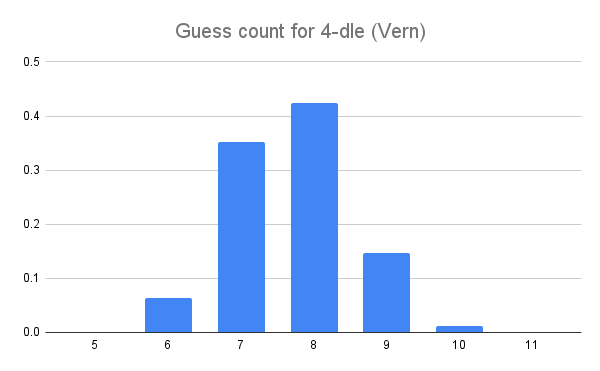
\includegraphics[scale=.33]{guess4_vern}}}%
 \qquad
 \subfloat[\centering frequency of openers]{{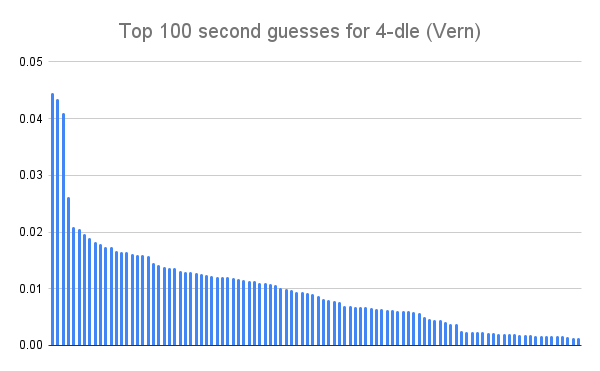
\includegraphics[scale=.33]{second4_vern}}}%
 \caption{4-dle results on 10000 random answer sets (Vern)}%
\end{figure}

\begin{figure}[!htb]
 \centering
 \subfloat[\centering last subpuzzle solved]{{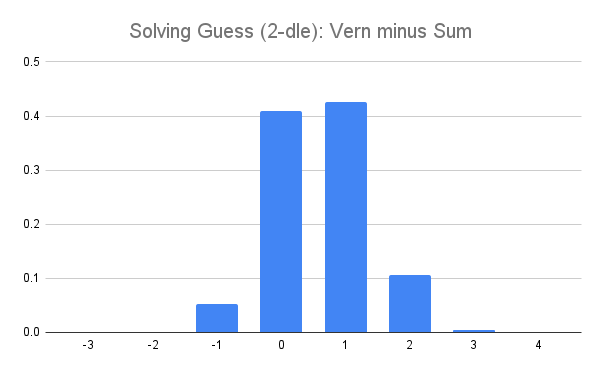
\includegraphics[scale=.33]{last_guess_comparison_4} }}%
 \qquad
 \subfloat[\centering first subpuzzle solved]{{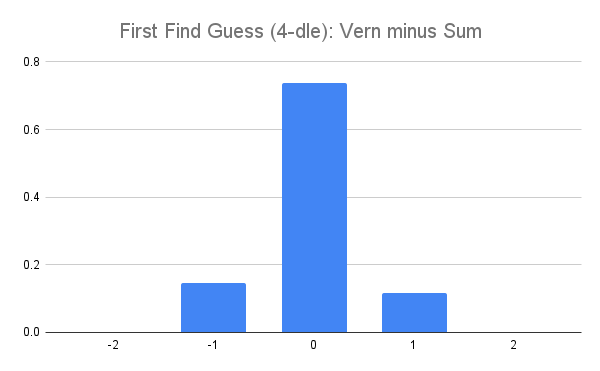
\includegraphics[scale=.33]{first_guess_comparison_4} }}%
 \caption{Comparison of Vern and Sum algorithms on 4-dle}%
\end{figure}


\begin{itemize}
\item Expected Guess Count: 7.6927 (vs. sum strategy: 7.0954)
\item Opener 1: \emph{soare, clint} (.0446)
\item Opener 2: \emph{soare, lemel} (.0434)
\item Opener 3: \emph{soare, thilk} (.041)
\item Opener 4: \emph{soare, clink} (.0262)
\item Prevalence of top four openers: (0.1552). 
\end{itemize}

Observations:
\begin{itemize}
\item The right tail of solution length increases; more than 1\% of Vern's Gambit solutions exceed the legal limit of 9 (N+5) guesses for N = 4.
\item The top three second moves have similar probability, as opposed to one dominant opening.
\item While 41\% of the time, the sum and min methods yield the same guess count, a full 53\% see the sum method winning (Fig 12a).  
\end{itemize}

\subsection{Octordle (8-dle) under Vern's gambit}

\begin{center}
\begin{tabular}{ |c|c|c| }
 \hline
guesses & count & proportion \\
 \hline
9 & 12 & 0.0012 \\
10 & 1430 & 0.143 \\
11 & 3766 & 0.3766 \\
12 & 3269 & 0.3269 \\
13 & 1273 & 0.1273 \\
14 & 218 & 0.0218 \\
15 & 31 & 0.0031 \\
16 & 1 & 0.0001 \\
 \hline
\end{tabular}
\end{center}

\begin{figure}[!htb]
 \centering
 \subfloat[\centering guesses required]{{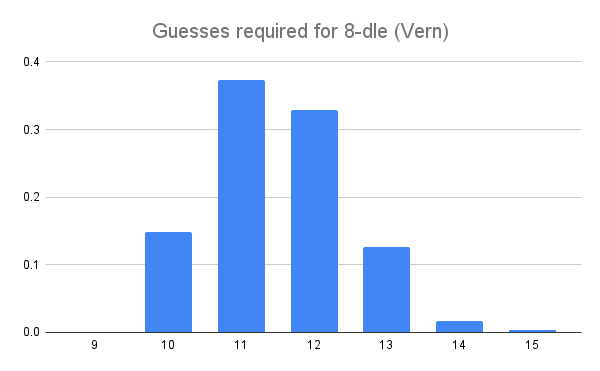
\includegraphics[scale=.33]{guess8_vern}}}%
 \qquad
 \subfloat[\centering frequency of openers]{{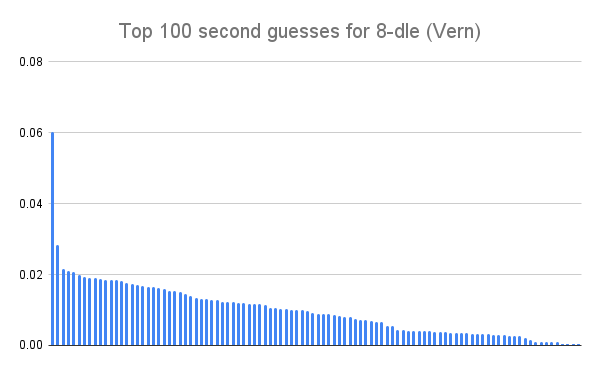
\includegraphics[scale=.33]{second8_vern}}}%
 \caption{8-dle results on 10000 random answer sets (Vern)}
\end{figure}

\begin{figure}[!htb]
 \centering
 \subfloat[\centering last subpuzzle solved]{{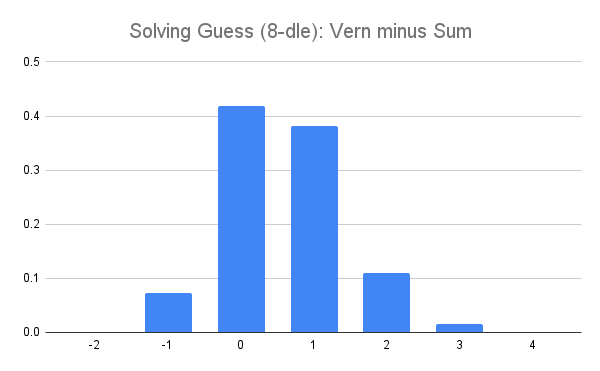
\includegraphics[scale=.33]{last_guess_comparison_8} }}%
 \qquad
 \subfloat[\centering first subpuzzle solved]{{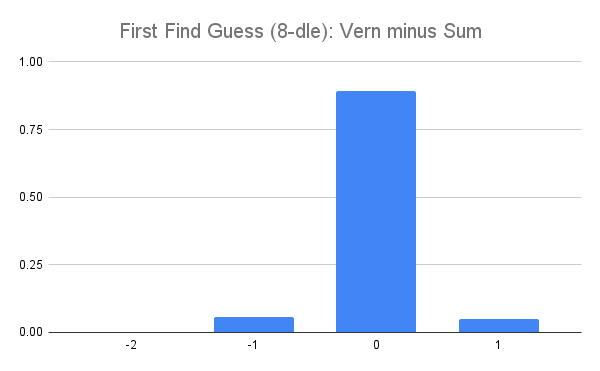
\includegraphics[scale=.33]{first_guess_comparison_8} }}%
 \caption{Comparison of Vern and Sum algorithms on 8-dle}%
\end{figure}


\begin{itemize}
\item Expected Guess Count: 10.9403 (vs. sum strategy: 11.5144)
\item Opener 1: \emph{soare, lemel} (.0602)
\item Opener 2: \emph{soare, tichy} (.0284)
\item Opener 3: \emph{soare, butch} (.0217)
\item Opener 4: \emph{soare, cloud} (.0.0210)
\item Prevalence of top four openers: (0.1313). 
\end{itemize}

Observations:
\begin{itemize}
\item More than 2\% of Vern's Gambit solutions exceed the limit of 13 (N+5) guesses for N = 8.
\item The sum method beats min on 51\% of trials (Fig 14a).  
\item The advantage of the min method (finding the first puzzle quickly) seem to diminish (or be swept into the ``tie'' category as both methods capitalize early).
\end{itemize}


\textbf{In summary, the sum method seems to outpace the min method in most metrics}, especially as N increases.

\section{Remaining Questions}

Many questions remain for me. Given the volume of armchair math written about Wordle, I can only assume others are asking (and possibly answering!) these questions also.

\begin{itemize}
\item Other than relative monotonicity, what is the link between the measure of entropy and expected moves remaining? Given that the ``branching factor'' changes so much through the search space, it does not seem so simple as, say, doing a binary search with a coin.
\item Mastermind, whose guess-and-answer mechanic Wordle adopted, is an entirely ``smooth'' space: every guess is legal, and every combination of ``letters'' (colors in Mastermind's case) is possible (and equally so). Would this kind of result fall out of Mastermind? Donald Knuth built a minimax-based (search) algorithm to solve Mastermind, detailed here \cite{5}. The answer to this question indicates whether our results say more about the algorithm or the dictionary.
\item There are certainly other algorithms to solve n-dle. Healy \cite{1} mentioned looking two moves ahead and estimating the conditional entropy there (computationally expensive), as well as limiting guesses to only possible answers, both of which can perform better.
\end{itemize}

\begin{thebibliography}{9}

\bibitem{1}
Alex Healy \emph{On Optimal Strategies for Wordle}, \url{http://www.alexhealy.net/papers/wordle.pdf}.
\bibitem{2}
Claude Shannon (1948) \emph{A Mathematical Theory of Communication}. Bell System Technical Journal 27, 379-423.
\bibitem{3}
Thomas M. Cover; Joy A. Thomas (1991). \emph{Elements of Information Theory}, retrieved from \url{https://en.wikipedia.org/wiki/Entropy_(information_theory)}
\bibitem{4}
Wikipedia: \url{https://en.wikipedia.org/wiki/Huffman_coding}
\bibitem{5}
Knuth, Donald (1976-1977). \emph{The Computer as Master Mind}. J. Recr. Math (9): 1-6.
\end{thebibliography}
\end{document}
